\documentclass[answer]{cphos}

\cphostitle{CPHOS物理竞赛联考}
\cphossubtitle{理论试题}

\setscorecheck{true}

\begin{document}

\begin{problem}[50]{卫星绕地} 

\begin{problemstatement}
在普通的二体开普勒运动中，两天体的相对运动轨迹是一个不变的椭圆；当存在外界扰动（摄动）时，这个椭圆变为随时间变化的。
更具体地，将小天体（质量为$m$）相对大天体（质量为$M$）的瞬时运动视作椭圆运动，而用椭圆的参数与小天体在椭圆上的位置参数（统称为轨道根数）描述小天体的瞬时运动。当存在摄动时，将小天体受力$\vec{ F}$分解为引力$\vec{P}=-\frac{GMm\vec{e}_r}{r^2}$与摄动力$\vec{R}$，即$\vec{F}=\vec{P}+\vec{R}$，并利用运动方程求出在$\vec{R}$摄动下轨道根数的变化。

选择地球与人造卫星为考虑的两个天体，建立参考坐标系如下图，其中原点$O$为地球中心，$xyz$系的方向待定。
令小天体位于$C$点，以$C$为原点建立随体坐标系$r\theta n$，其中$r$轴沿$\vec{OC}$方向，$n$轴沿轨道平面法向，$\theta$轴方向与$rn$平面垂直。

\begin{figure}[H]
	\centering
	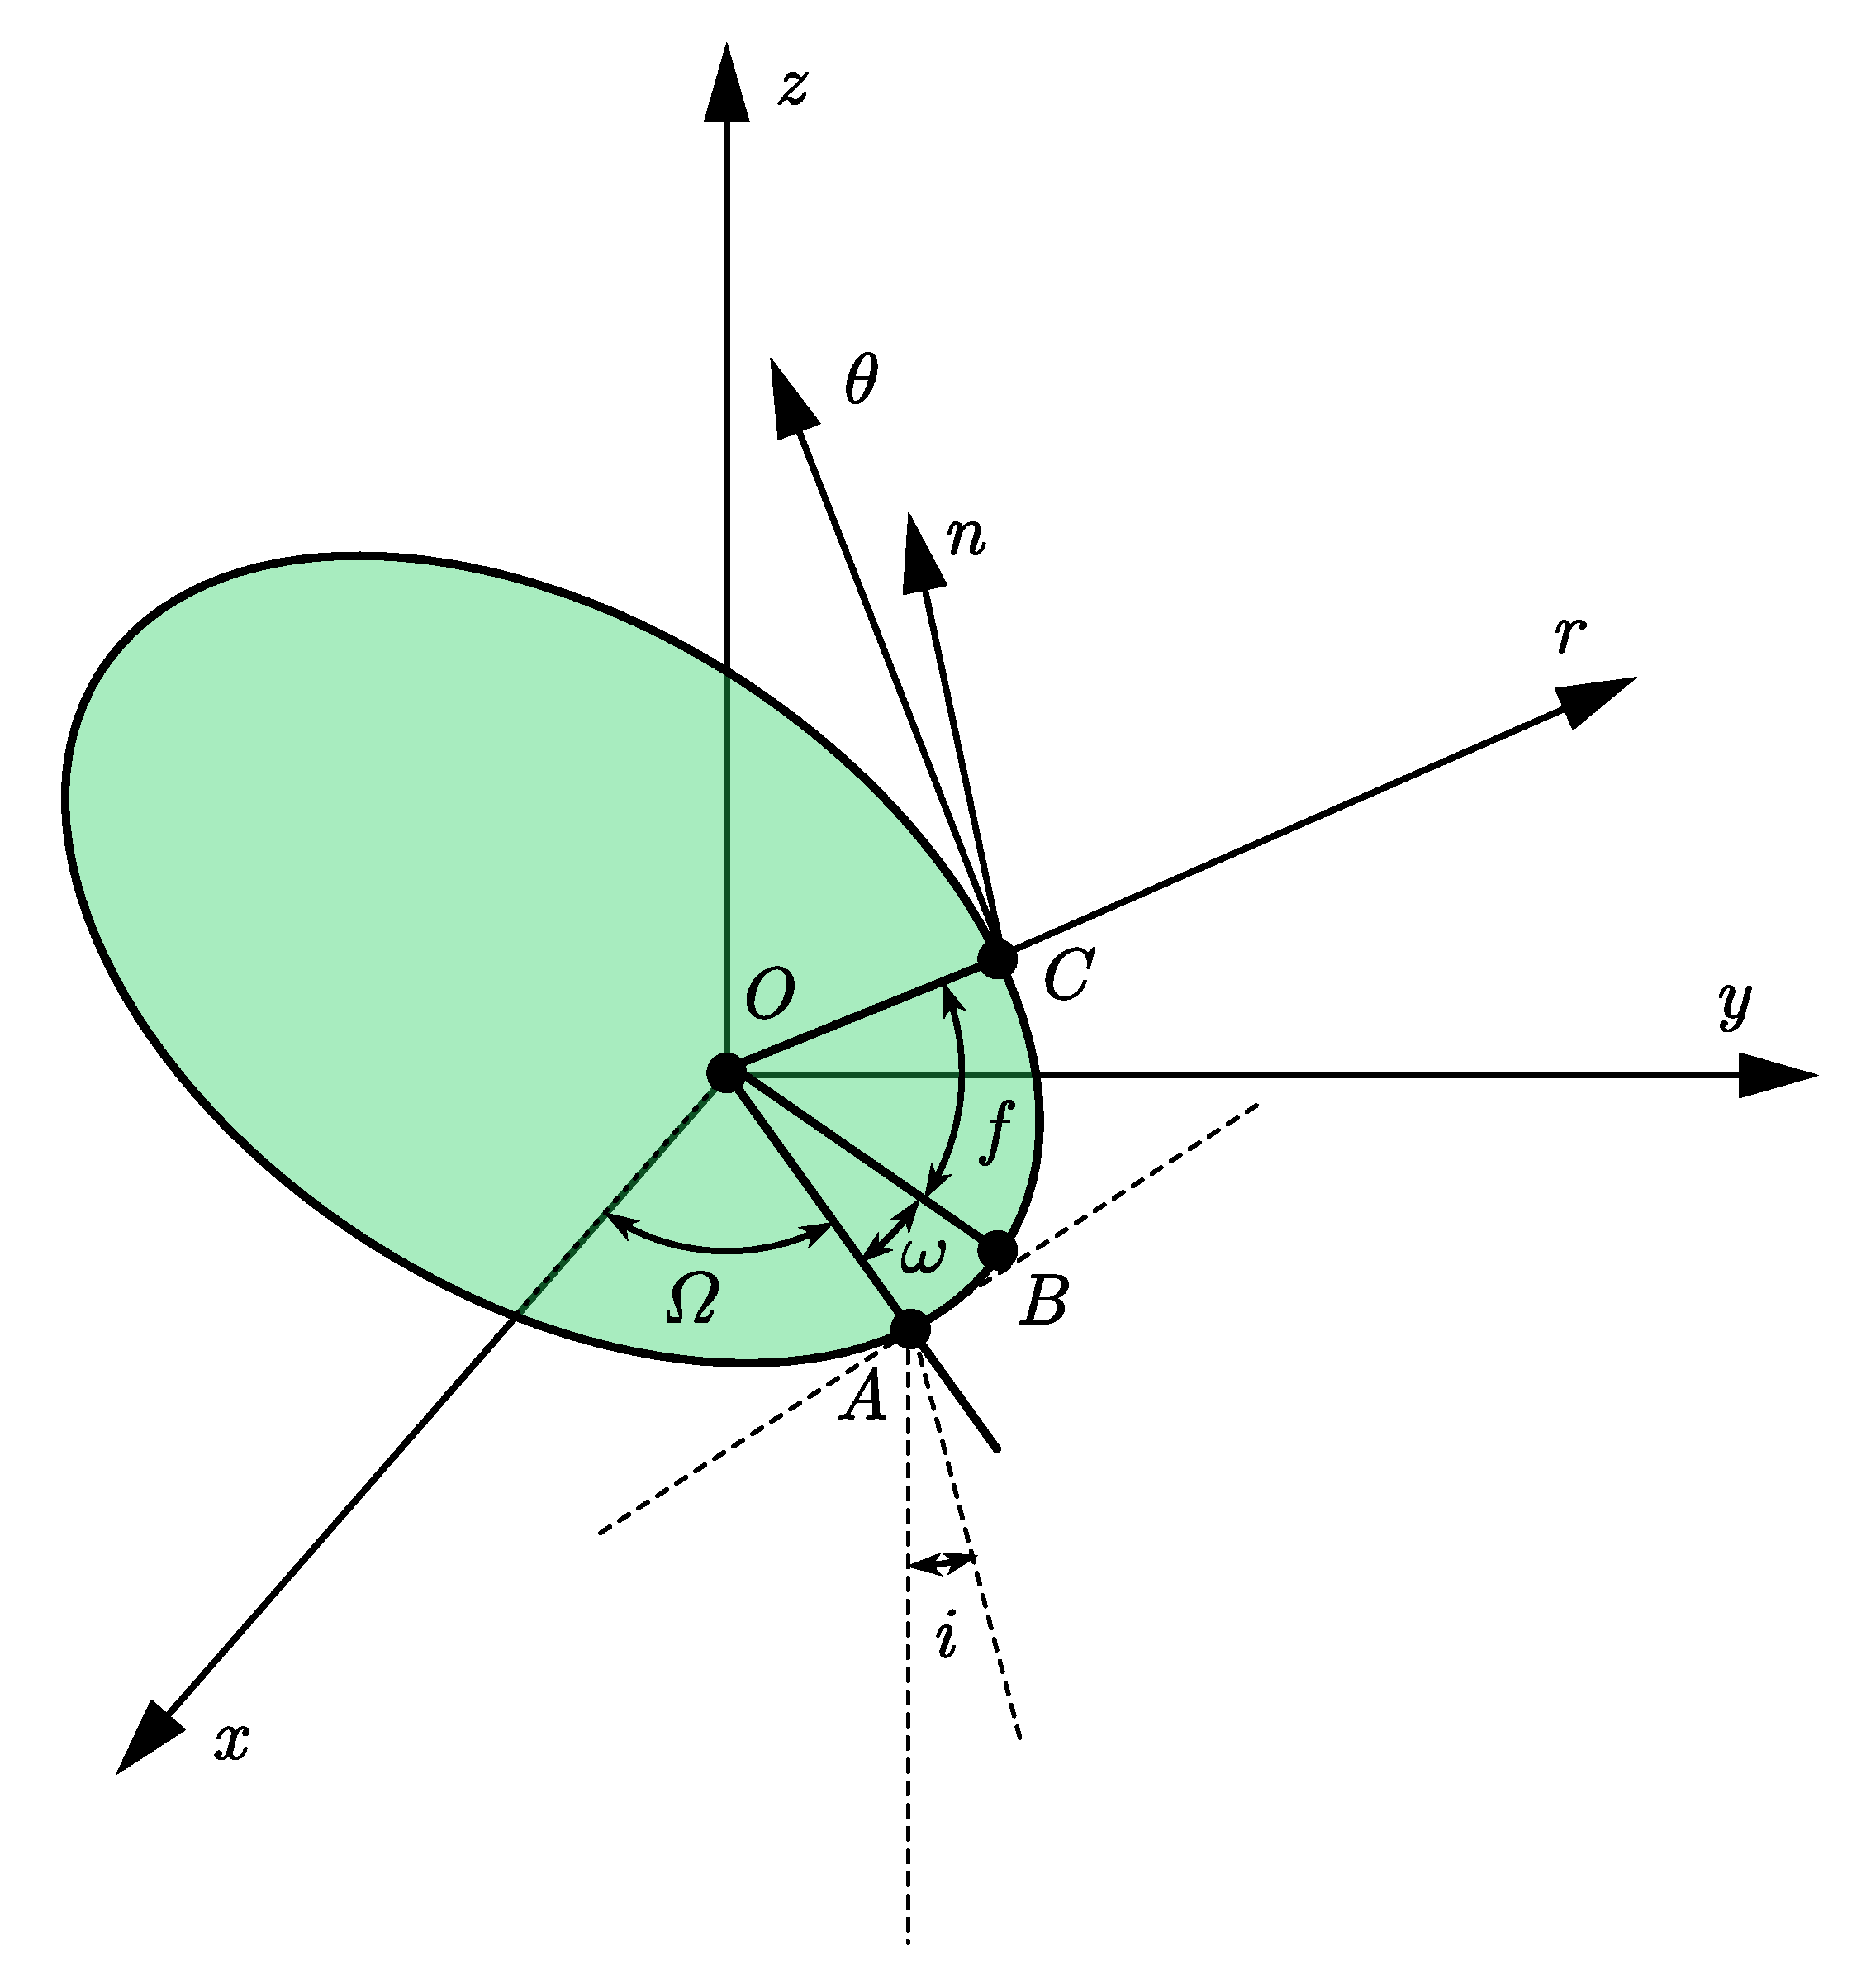
\includegraphics[width=0.5\textwidth]{assets/orbit.pdf}
	\caption{椭圆轨道及参数}
	\label{fig:e}
\end{figure}

\subq{1} 显然，轨道根数共有6个。取$\left(a, e, i, \varOmega, \omega, f\right)$为一组轨道根数，其中$a$为轨道半长轴，$e$为轨道离心率，
$i$为轨道平面与$xy$平面的夹角；作轨道平面与$xy$平面的交线$OA$，$\varOmega$为$OA$与$x$轴的夹角，令轨道近心点为$B$，$\omega$为$OB$与$OA$的夹角，
$f$为$OB$和$OC$的夹角。

\subsubq{1.1}给出前四个轨道根数与能量$E$，角动量$\vec L=\left(L_x,L_y,L_z\right)$的关系。提示：利用角动量与$n$轴平行的特点。

\subsubq{1.2}求出此时六个轨道根数的时间导数，结果可以包含六个轨道根数本身与摄动力在$r\theta n$系的分量$\left(R_r, R_\theta, R_n\right)$。近似到摄动力的一阶。

\subq{2} 
人造卫星在黄道面（地球的轨道平面）上绕地球沿$e\sim 10^{-4}$的近圆轨道运行，轨道高度为$h=500\text{~km}$。为计算简便，认为月球、地球的公转运动都是恒定的椭圆运动，此时月球有$\omega_m=\frac{\uppi}{2}$，地球是完美的球体。\\
已知太阳质量$M_S=1.989\times10^{30}\text{~kg}$，日地平均距离$R_S=1.496\times10^{8}\text{~km}$，
月球质量$M_m=7.342\times10^{22}\text{~kg}$，地月平均距离$R_m=3.844\times10^{5}\text{~km}$，
月球轨道的离心率$e_m=0.0549$，地球轨道的离心率$e_E=0.0167$，月球轨道平面与黄道面夹角$\phi=0.0898\text{~rad}$，地球质量$M_E=5.972\times10^{24}\text{~kg}$，地球半径$R_E=6378\text{~km}$。

\subsubq{2.1}回答：月球的摄动效应和太阳的哪个更强？本问只需要做估算。

\subsubq{2.2}只考虑上问中更强的效应，以黄道面作为$xy$平面，前三个轨道根数中变化最明显的（对应于$\left(\frac{\delta a}{a}, \delta e, \delta i\right)$中最大的）是哪个？并求出它的变化量。长度量纲取$\text{km}$，角度采用弧度制，保留一位有效数字。

\subq{3} 在近地大气中，人造卫星受到方向与速度相反的微弱阻力，大小正比于$v ^n$。在按周期平均的意义下，它的半长轴$a$，离心率$e$会如何变化？已知$e\leq\frac{1}{\sqrt{2}}$。（回答：变大/变小/不变）\\

\noindent 提示，你可能会用到以下公式：
\begin{equation}
	\int_{0}^{2\uppi}\sin^2 x \,\mathrm{d}x=\uppi,\quad
	\int_{0}^{2\uppi}\frac{A+\cos x}{\left(1+A\cos x\right)^2}\,\mathrm{d}x=0
\end{equation}

\end{problemstatement}

% === 解答 ===

\begin{solution}

\solsubq{1}{21}
\solsubsubq{1.1}{4}
当能量为$E$，角动量大小为$L$，熟知开普勒运动的解：
\begin{equation}
	a=-\frac{GMm}{2E} \eqtagscore{1}{1} 
\end{equation}
\begin{equation}
	e=\sqrt{1+\frac{2EL^2}{G^2M^2m^3}} \eqtagscore{2}{1}
\end{equation}
由几何关系可得：
\begin{equation}
	i=\arccos\left(\frac{L_z}{L}\right) \eqtagscore{3}{1}
\end{equation}
\begin{equation}
	\varOmega=-\arctan\left(\frac{L_x}{L_y}\right) \eqtagscore{4}{1}
\end{equation}
\solsubsubq{1.2}{17}
此时位置与速度：
\begin{equation}
	r=\frac{a\left(1-e^2\right)}{1+e\cos f} \eqtagscore{5}{1}
\end{equation}
\begin{equation}
	\dot{f}_0=\frac{L}{mr^2}=\sqrt{\frac{GM}{a^3\left(1-e^2\right)^3}}\left(1+e\cos f\right)^2 \eqtagscore{6}{1}
\end{equation}
这里，$\dot{f}_0$并非$f$的变化率，而只是瞬时标架下的椭圆运动角速度。
\begin{equation}
	\dot{r}=\frac{\partial{r}}{\partial{f}}\dot{f}_0=\sqrt{\frac{GM}{a\left(1-e^2\right)}}e\sin f \eqtagscore{7}{1}
\end{equation}
由功能原理和角动量定理得到$E, \vec L$的变化率
\begin{equation}
	\dot{E}=R_{r}\dot{r}+R_{\theta}r\dot{f}_0 \eqtagscore{8}{1}
\end{equation}
\begin{equation}
	\frac{\mathrm{d}\vec{L}}{\mathrm{d}t}=\vec{r}\times\vec{R}  \eqtag{9}
\end{equation}
即
\begin{equation}
	\frac{\mathrm{d}L_x}{\mathrm{d}t} = r\left[R_\theta \sin i \sin \varOmega + R_n \sin\left(\omega + f\right) \cos \varOmega + R_n \cos\left(\omega + f\right) \cos i \sin \varOmega\right] \eqtagscore{10}{1}
\end{equation}

\begin{equation}
	\frac{\mathrm{d}L_y}{\mathrm{d}t} = r\left[-R_\theta \sin i \cos \varOmega + R_n \sin\left(\omega + f\right) \sin \varOmega - R_n \cos\left(\omega + f\right) \cos i \cos \varOmega\right] \eqtagscore{11}{1}
\end{equation}

\begin{equation}
	\frac{\mathrm{d}L_z}{\mathrm{d}t} = r\left[R_\theta \cos i - R_n \cos\left(\omega + f\right) \sin i\right] \eqtagscore{12}{1}
\end{equation}
\begin{equation}
	\dot{L}=rR_{\theta} \eqtagscore{13}{1}
\end{equation}
注意到
\begin{equation}
	\frac{\dot{a}}{a}=-\frac{\dot{E}}{E} \eqtag{14}
\end{equation}
\begin{equation}
	\frac{2e\dot{e}}{e^2-1}=\frac{\dot{E}}{E}+\frac{2\dot{L}}{L} \eqtag{15}
\end{equation}

可得
\begin{equation}
	\frac{\mathrm{d}a}{\mathrm{d}t} = \frac{2a^{\frac{3}{2}}}{\sqrt{GMm^2\left(1-e^2\right)}} \left[R_r e \sin f + R_\theta \left(1+e \cos f\right)\right] \eqtagscore{16}{1} \label{eq:1.1}
\end{equation}

\begin{equation}
	\frac{\mathrm{d}e}{\mathrm{d}t} = \sqrt{\frac{a\left(1 - e^2\right)}{GMm^2}} \left[R_r \sin f + R_\theta \left(\cos f + \frac{e+\cos f}{1+e\cos f}\right)\right] \eqtagscore{17}{1}  \label{eq:1.2}
\end{equation}
同理有
\begin{equation}
	\frac{\mathrm{d}i}{\mathrm{d}t} =\sqrt{\frac{a\left(1 - e^2\right)}{GMm^2}}\frac{R_n\cos\left(\omega+f\right)}{1+e\cos f}  \eqtagscore{18}{1} \label{eq:1.3}
\end{equation}
\begin{equation}
	\frac{\mathrm{d}\varOmega}{\mathrm{d}t} =\sqrt{\frac{a\left(1 - e^2\right)}{GMm^2}}\frac{R_n\sin\left(\omega+f\right)}{\left(1+e\cos f\right)\sin i}  \eqtagscore{19}{1} \label{eq:1.4}
\end{equation}
对
\begin{equation}
	\frac{L^2}{GMm^2}=r\left(1+e\cos f\right) \eqtag{20} 
\end{equation}
求导得到
\begin{equation}
	\dot{f}=\dot{f}_0 + \frac{\dot{e}}{e \tan f} - \frac{2\dot{L}\left(1+e\cos f\right)}{Le\sin f} \eqtagscore{21}{1}
\end{equation}
即
\begin{equation}
	\frac{\mathrm{d}f}{\mathrm{d}t}=\sqrt{\frac{GM}{a^3\left(1-e^2\right)^3}}\left(1+e\cos f\right)^2+ \sqrt{\frac{a\left(1 - e^2\right)}{GMm^2}}\frac{1}{e}\left(R_r\cos f - R_{\theta}\sin f\frac{2+e\cos f}{1+ e\cos f}\right) 
	\eqtagscore{22}{1} \label{eq:1.5}
\end{equation}
下面计算$\dot{\omega}$：
\begin{multisol}
	\item
	由
	\begin{equation}
		\begin{pmatrix}
			x \cos \varOmega + y \sin \varOmega \\
			-x \sin \varOmega + y \cos \varOmega \\
		\end{pmatrix} = \begin{pmatrix}
			r \cos\left(\omega + f\right) \\
			r \sin\left(\omega + f\right) \cos i \\
		\end{pmatrix} \eqtagscore{23}{1}
	\end{equation}
	对第一式求导可得：
	\begin{equation}
		-r\sin\left(\omega+f\right)\dot{\varOmega} \cos i=r\sin\left(\omega+f\right)\left(\dot{\omega}+\left(\dot{f}-\dot{f}_0\right)\right) \eqtagscore{24}{1}
	\end{equation}
	即
	\begin{equation}	
		\frac{\mathrm{d}\omega}{\mathrm{d}t}=-\sqrt{\frac{a\left(1 - e^2\right)}{GMm^2}}\left[\frac{R_n\sin\left(\omega+f\right)}{\left(1+e\cos f\right)\tan i}+\frac{1}{e}\left(R_r\cos f - R_{\theta}\sin f\frac{2+e\cos f}{1+ e\cos f}\right)\right]
		\eqtagscore{25}{1} \label{eq:1.6}
	\end{equation}	
	\item
	定义隆格-楞次矢量
	\begin{equation}
		\vec{e}=\frac{\vec{p}\times\vec{L}}{GMm^2}-\vec{e_r} \eqtag{23*}
	\end{equation}
	其中，$\vec{p},\vec{L}$为动量和角动量。可以证明其恒与$OB$平行，值为$e$。
	\begin{equation}
		\frac{\mathrm{d}\vec{e}}{\mathrm{d}t}=\frac{\vec{R}\times\vec{L}+\vec{p}\times\frac{\mathrm{d}\vec{L}}{\mathrm{d}t}}{GMm^2}
		\eqtagscore{24*}{1}
	\end{equation}
	\begin{equation}
		\omega=\arccos\left(\frac{e_x\cos\varOmega+e_y\sin\varOmega}{e}\right) \eqtagscore{25*}{1}
	\end{equation}
	求导可以得到
	\begin{equation}	
		\frac{\mathrm{d}\omega}{\mathrm{d}t}=-\sqrt{\frac{a\left(1 - e^2\right)}{GMm^2}}\left[\frac{R_n\sin\left(\omega+f\right)}{\left(1+e\cos f\right)\tan i}+\frac{1}{e}\left(R_r\cos f - R_{\theta}\sin f\frac{2+e\cos f}{1+ e\cos f}\right)\right]
		\eqtagscore{26*}{1}
	\end{equation}	
\end{multisol}

\solsubq{2}{20}
\solsubsubq{2.1}{4}
轨道的摄动需要考虑相对地心的潮汐力：
\begin{equation}
	\vec{R}=\vec{r}\cdot\nabla\vec{P}'\sim\frac{GMmr}{R^3} \eqtagscore{27}{1}
\end{equation}
式中，$P'$为摄动天体（月球/太阳）对卫星的引力。
计算
\begin{equation}
	\frac{R_S}{r} \sim \frac{M_S}{R_S^3}\approx6\times10^5 \text{~kg/km}^3 \eqtag{28}
\end{equation}
\begin{equation}
	\frac{R_m}{r} \sim \frac{M_m}{R_m^3}\approx1.3\times10^6 \text{~kg/km}^3 \eqtag{29}
\end{equation}
\begin{equation}
	R_S<R_m \eqtag{30}
\end{equation}

因此月球的摄动效应更强。\addtext{说明月球摄动效应更强}{3}

\solsubsubq{2.2}{16}
在以下的计算中，$e_m, \phi$将被当作一阶小量，$e$视作二阶小量。\\
以地心为原点，为避免$i=0$导致的发散，以月球轨道平面为$xy$平面，地心与月球近心点连线为$x$轴方向，则在此坐标系中初态的轨道根数为$\left(r, e, \phi, 0, \omega_0, f_0\right)$。我们下面先借用符号表示此坐标系中的轨道根数，在最后换到原系中。\\
设月球的位矢为$\vec{\rho}$，卫星的位矢为$\vec{r}$，考虑潮汐力的一阶展开，则卫星受到的摄动力为：
\begin{equation}
	\vec{R}=\left(\vec{r}\cdot\nabla\right)\frac{GM_{m}m\left(\vec{\rho}-\vec{r}\right)}{\left|\vec{\rho}-\vec{r}\right|^3}=GM_{m}m\left(-\frac{\vec{r}}{\rho^3}+\frac{3\vec{\rho}\left(\vec{r}\cdot\vec{\rho}\right)}{\rho^5}\right) \eqtagscore{31}{2} \label{eq:2.1}
\end{equation}
容易看出，$\frac{r}{\rho}$是和$e_m, \phi$同阶的小量。\\
对$e_m, \phi, e$作恰当的近似，写出：
\begin{equation}
	\vec{\rho}=\frac{a_m\left(1-e_m^2\right)}{1+e_m\cos\theta}\left(\cos\theta,\sin\theta,0\right)\approx\frac{R_m}{1+e_m\cos\theta}\left(\cos\theta,\sin\theta,0\right)
	\eqtag{32}
\end{equation}
\begin{equation}
	\begin{aligned}
		\vec{r}&=r\left(\cos\phi\sin\left(\omega+f\right),-\cos\left(\omega+f\right),\sin\phi\sin\left(\omega+f\right)\right)\\
		&=r\left(\sin\left(\omega+f\right),-\cos\left(\omega+f\right),\phi\sin\left(\omega+f\right)\right)
	\end{aligned}\eqtag{33}
\end{equation}
式中$r=R_E+h$。\\ 
代入\ref{eq:2.1}式，再利用：
\begin{equation}
	\begin{aligned}
		&\vec{e_r}=\left(\sin\left(\omega+f\right),-\cos\left(\omega+f\right),\phi\sin\left(\omega+f\right)\right),\\
		&\vec{e_{\theta}}=\left(\cos\left(\omega+f\right),\sin\left(\omega+f\right),\phi\sin\left(\omega+f\right)\right),\\
		&\vec{e_n}=\left(-\phi,0,1\right)
	\end{aligned} \eqtagscore{34}{1}
\end{equation}

\begin{equation}
	\begin{aligned}
		&R_r=\vec{R}\cdot{e_r},\\
		&R_\theta=\vec{R}\cdot{e_{\theta}},\\
		&R_n=\vec{R}\cdot{e_n}
	\end{aligned} \eqtag{35}
\end{equation}
得到：
\begin{equation}
	\begin{aligned}
		&R_r=\frac{GM_{m}mr\left(1+e_m\cos\theta\right)^3}{R_m^3}\left(-1+3\sin^2\left(\omega+f-\theta\right)\right)\\
		&R_\theta=\frac{3GM_{m}mr\left(1+e_m\cos\theta\right)^3}{R_m^3}\sin\left(\omega+f-\theta\right)\cos\left(\omega+f-\theta\right)\\
		&R_n=-\frac{3GM_{m}mr\left(1+e_m\cos\theta\right)^3\phi\cos\theta\sin\left(\omega+f-\theta\right)}{R_m^3}
	\end{aligned} \eqtagscore{36}{3}
\end{equation}
首先计算$\frac{\mathrm{d}\varOmega}{\mathrm{d}t}$。由\ref{eq:1.4}，取最低阶近似得到：
\begin{equation}
	\frac{\mathrm{d}\varOmega}{\mathrm{d}t} \approx-\frac{3M_{m}(1+e_m\cos\theta)^3\cos\theta\cos(\omega+f-\theta)\sin(\omega+f)}{R_m^3}\sqrt{\frac{Gr^3}{M_{E}}} \eqtagscore{37}{1}
\end{equation}
由于
\begin{equation}
	\dot{\omega}+\dot{f}=\dot{f}_0-\dot{\varOmega}\cos i\approx\dot{f}_0-\dot{\varOmega} \eqtag{38}
\end{equation}
而
\begin{equation}
	\dot{f}_0\approx\sqrt{\frac{GM_E}{r^3}}\eqtag{39}
\end{equation}
第二项与第一项之比为
\begin{equation}
	\frac{\dot{\varOmega}}{\dot{f}_0}\sim\frac{M_{m}r^3}{M_{E}R_{m}^3}\approx7\times10^{-8} \eqtagscore{40}{1}
\end{equation}
所以可以认为$\omega+f$的变化率恒定。
对$\omega+f$取平均，保留到最低阶，
\begin{equation}
	\left\langle\frac{\mathrm{d}\varOmega}{\mathrm{d}t}\right\rangle=-\frac{3M_{m}(1+e_m\cos\theta)^3\cos^2\theta}{2R_m^3}\sqrt{\frac{Gr^3}{M_{E}}} \eqtag{41}
\end{equation}
再对$\theta$取平均，
\begin{equation}
	\left\langle\frac{\mathrm{d}\varOmega}{\mathrm{d}t}\right\rangle=-\frac{3M_{m}}{4R_m^3}\sqrt{\frac{Gr^3}{M_{E}}} \eqtagscore{42}{1}
\end{equation}
经过一年的变化量：
\begin{equation}
	\delta\varOmega=\dot{\varOmega}\times(365\times86400\text{~s})=2\times10^{-3}\text{~rad} \eqtagscore{43}{1}
\end{equation}
同理，可以得到
\begin{equation}
	\left\langle\frac{\mathrm{d}i}{\mathrm{d}t}\right\rangle\approx 0 \eqtagscore{44}{1}
\end{equation}
由\ref{eq:1.1}，
\begin{equation}
	\frac{\frac{\mathrm{d}a}{\mathrm{d}t}}{a}= 2\sqrt{\frac{r}{GM_Em^2}} [R_r e \sin f + R_\theta (1+e \cos f)] \eqtag{45}
\end{equation}
由于$\bar R_\theta\approx0$，故
\begin{equation}
	\overline{\frac{\frac{\mathrm{d}a}{\mathrm{d}t}}{a}}\sim e\dot{\varOmega} \eqtagscore{46}{1}
\end{equation}
由\ref{eq:1.2}，
\begin{equation}
	\frac{\mathrm{d}e}{\mathrm{d}t} = \sqrt{\frac{r}{GM_Em^2}} \left[R_r \sin f + R_\theta \left(\cos f + \frac{e+\cos f}{1+e\cos f}\right)\right] \eqtag{47}
\end{equation}
由\ref{eq:1.5}，
\begin{equation}
	\dot{f}-\dot{f}_0=\sqrt{\frac{r}{GM_Em^2}}\frac{1}{e}\left(R_r\cos f - R_{\theta}\sin f\frac{2+e\cos f}{1+ e\cos f}\right) \eqtag{48}
\end{equation}
计算
\begin{equation}
	\frac{\dot{f}-\dot{f}_0}{\dot{f}_0}\sim \frac{M_{m}r^3}{eM_{E}R_{m}^3}\approx7\times10^{-4}  \eqtagscore{49}{1} \label{eq:2.2}
\end{equation}
则
\begin{equation}
	\dot{\omega}=-\dot{\varOmega}\cos i-\left(\dot{f}-\dot{f}_0\right) \eqtag{50}
\end{equation}
为量级$10^{-4}\dot{f}_0$的小量。\\
则$\overline{R_r\sin\left(\omega+f-\omega\right)}\approx0, \overline{R_\theta\cos\left(\omega+f-\omega\right)}\approx0$
\begin{equation}
	\overline{\frac{\mathrm{d}e}{\mathrm{d}t}}\sim 10^{-4}\dot{\varOmega} \eqtagscore{51}{1}
\end{equation}
\begin{equation}
	\overline{\dot{\omega}}\sim\dot{\varOmega} \eqtagscore{52}{1}
\end{equation}
由于 $\dot{\omega}$ 不引起 $i$ 的变化，所以有：
\begin{equation}
	\delta i\approx\phi\,\delta\varOmega\approx2\times10^{-4}\text{~rad} \eqtagscore{53}{1}
\end{equation}
为三者中变化最明显的量。

\solsubq{3}{9}
总能量变小，所以$a$会变小。\addtext{说明a变小}{1}
式\ref{eq:1.2}中摄动力改写为正比形式：
\begin{equation}
	\begin{aligned}
		& R_r\propto -v^{n-1}\dot{r} \propto -\left(1+e^2+2e\cos f\right)^{\frac{n-1}{2}}e\sin f\\
		& R_\theta \propto -v^{n-1}r\dot{f}_0 \propto -\left(1+e^2+2e\cos f\right)^{\frac{n-1}{2}}\left(1+e\cos f\right) 
	\end{aligned}
	\eqtagscore{54}{2}
\end{equation}
代入得到

\begin{equation}
	\frac{\mathrm{d}e}{\mathrm{d}f}\propto-\frac{\left(1+e^2+2e\cos f\right)^{\frac{n-1}{2}}\left(e+\cos f\right)}{\left(1+e\cos f\right)^2} \eqtagscore{55}{1}
\end{equation}

特别地，$n=1$时，由题给积分式可得$\int_{0}^{2\uppi} \frac{\mathrm{d}e}{\mathrm{d}f}\,\mathrm{d}f=0$。
由于$\cos f>0$时
\begin{equation}
	\frac{\left(e+\cos f\right)}{\left(1+e\cos f\right)^2}-\frac{\left(e-\cos f\right)}{\left(1-e\cos f\right)^2}=\frac{2\cos f\left(1+e^2\cos^2 f-2e^2\right)}{\left(1-e^2\cos^2 f\right)^2}\geq0 \eqtag{56}
\end{equation}
当$n>1$时，速度项会为$\cos f>0$的积分区域乘上一个较大的因子，$n<1$时，速度项会为$\cos f>0$的积分区域乘上一个较小的因子，
因此$n>1$时$e$会变小，$n<1$时$e$会变大，$n=1$时$e$不变。\addtext{说明$n=1$时$e$不变}{1}\addtext{$n>1$时$e$变小，$n<1$时$e$变大}{4}

\scoring

% === 题目附录（可选） ===
\begin{problemappendix}
	本题考虑的不是实际情况，事实上对于近地轨道卫星，题中考虑的摄动太小，地球的四极矩导致的$J_2$摄动项、空气阻力的摄动都远大于月球摄动；月球轨道的周期变化也没有考虑。
\end{problemappendix}

\end{solution}

\end{problem}

\end{document}